\documentclass[]{article}
\usepackage{times}

% numbers option provides compact numerical references in the text. 
\usepackage[numbers]{natbib}
\usepackage{multicol}
\usepackage[bookmarks=true]{hyperref}
\usepackage{graphics} % for pdf, bitmapped graphics files
\usepackage{graphicx}

\usepackage{amsmath,amssymb,latexsym,float,epsfig,subfigure,mathtools}
\usepackage{amsmath} % assumes amsmath package installed
\usepackage{amssymb}  % assumes amsmath package installed
\usepackage{lipsum}
\usepackage[export]{adjustbox}
\usepackage[normalem]{ulem} % underline
\usepackage{wrapfig}
\usepackage{multirow}
\usepackage{balance}
\usepackage{color}
\usepackage{url}
\usepackage{booktabs}
\usepackage{pifont}
\usepackage{longtable}
\newcommand{\norm}[1]{\left\lVert#1\right\rVert}


%opening
%\title{Research Notes}
%\author{Deepak E. Gopinath}
\title{}
\author{}

\begin{document}

\date{}
%\maketitle

%\section*{June 1 2017}
%
%Ideas for journal article: Extensions on the current disambiguation formalism. 
%
%The goal for the journal article is not just to have a full scale study but also to extend the formalism and possibly situate the problem within a broader theoretical framework. 
%
%The notion of \textit{inverse legibility} as introduced in the RSS paper might be equivalent to eliciting/producing actions that results in \textit{maximum information transfer} between the human and the robot. The difference between eliciting and producing is that the former is "forced" by the robot whereas the latter is voluntarily provided by the human. 
%
%That is, 
%\begin{enumerate}
%	\item Producing actions: Action produced by the human leads to increase of information transfer from the human to the robot: $a_h \rightarrow$ max information transfer.
%	\item ``Eliciting actions'': Actions by the robot will in turn elicit a subsequent action from the human that will then lead to maximum information transfer so that the intent inference is maximized. $a_r \rightarrow a_h \rightarrow $ max information transfer
%\end{enumerate}
%
%As an extension to the RSS confidence formalism, confidences have been treated as a dynamical system. By controlling the time constant of decay, the system designer can control how fast or slow the confidences change. The time constant in essence plays the role of a filter. However, this does not necessarily mean that the dynamical system has ``memory''. 
%
%Confidence functions, if normalized, may be interpreted as $P(g^t | \boldsymbol{x^t}, \boldsymbol{u_h^t})$. However, this is still ``memoryless'' since the current goal only depends on the current state and the user control command. 
%
%\section*{June 6 2017}
%
%The ``confidence'' measure currently does not have ``memory''. That is, confidence measures do not represent $P(g^t | \boldsymbol{x^t}, \boldsymbol{u_h^t},\boldsymbol{x^t}, \boldsymbol{u_h^{t-1}},\boldsymbol{x^{t-2}}, \boldsymbol{u_h^{t-2}},\dots)$
%
%The confidence measures themselves can be thought of as evolving according to a DS in which $u_h\cdot u_r$ is the ``control input'' to the dynamical system
%\begin{equation*}
%\dot{\boldsymbol{c}} = f(\boldsymbol{c}, u_h\cdot u_r)
%\end{equation*}
%
%What does it mean to have a dynamical system whose ``rate of change'' depends not only on the current state but also on a small segment of the past trajectory. That is, if $x$ denotes a single-dimensional variable then, 
%\begin{equation*}
%	\dot{x}(t) = f(x(s), u(s)) ~ s.t.~~ s \in [t-T, t] 
%\end{equation*}
%Is this the notion of infinite-dimensional dynamical systems? Is this the way a dynamical system with memory represented?
%
%Another possible way to represent ``memory'' would be to have the derivative depend on the integral of $x(t)$ from start time till time $t$. That is, 
%\begin{equation*}
%\dot{x}(t) = f(\int\limits_{0}^{t}x(s)ds, \int\limits_{0}^{t}u(s)ds )
%\end{equation*}
%
%\section*{June 7 2017}
%
%One of the key ideas that I have been toying with is the notion of characterizing human-robot interaction as information transfer between two dynamical? systems. For successful and seamless interaction, it becomes important for the two parties to ``understand'' each other in some way. 
%
%What exactly do we mean by ``understanding'' in this context? From the perspective of the robot, for example this might include understanding and inferring the underlying intent of the human or interpreting speech instruction and unambiguously grounding it to the world. From the perspective of the human, it might include understanding how the robot operates and making sense of the actions taken by the robot. 
%The concept of ``working'' together, sharing control etc., becomes more effective when communication between the two parties is enhanced. Or more specifically, actions performed by the two parties should lead to maximum information transfer/gain between them.
%
%Key ideas to understanding explore:
%\begin{enumerate}
%	\item Entropy/Mutual information gain
%	\item Transfer entropy
%	\item Optimal control for maximizing information gain
%\end{enumerate}
%
%If we treat the human and the robot as dynamical systems, is it possible to cast the problem of performing the appropriate action (by either party) maximizing information gain as an optimal control problem. Assistive actions performed by the robot, such as automated mode switches and switching autonomy levels, can in turn \textit{elicit} other actions from the humans which will result in enhanced intent inference. 
%
%In some limited sense, appropriate assistance schemes are those which will maximize such infomration transfer. It is possible that after the proper intent inference, different types of assistance paradigms may be activated to perform context/task-specific functionalities. 
%
%\section*{June 12 2017}
%
%Last week, I discovered a work by Dorsa Sadigh titled ``Information Gathering Actions over Human Internal State'' published in IROS 2016 and also RSS 2016 in the idea of a robot ``nudging/probing'' the human is explored. The premise of the problem is similar to mine in that, the authors are also trying to ``elicit'' informative responses \textit{from} the human would respond. The problem is situated within a POMDP framework in which the robot's reward structure essentially is the information gain on the belief that it has about the human's internal state. The experiments in the paper use an autonomous car probing to a human driver to see if the driver is attentive or distracted. 
%
%There are few assumptions made by the author which makes the formalism works. 
%\begin{enumerate}
%	\item The existence of a human reward structure. This is learned using IRL techniques from demonstrations. 
%	\item The human policy is a function of the robot's policy and the authors also assume that the human has access to the \textit{entire} robot policy \textit{a priori.}
%	\item The framework also assumes that the humans are responding to the robot's actions at every time step. The robot first takes an action, which then elicits a response from the human. The dynamics/transition matrix is a nested function which incorporates the effects of both the human control commands and the robot control command. 
%	\item an MPC framework is used to compute a sequence of robot control commands over a time horizon such that the robot's cumulative expected reward is maximized. The authors also derive a closed-form expression for a gradient that is used in the optimization procedure. This is similar to optimal control. Computing derivatives of cost function with respect to sequence of controls or a control curve (in case of continuous time). 
%\end{enumerate}
%
%How similar/dissimilar is this work from what I am thinking about?
%
%The core idea is essentially the same. In fact, the last paragraph of the introduction contains a statement very similar to what I had written down in my notes even before I knew about this work. 
%
%The mathematical formalism they have introduced is sound and conforms to standard approaches. However, there are numerous components (IRL learning, MDP solvers) that need to come together for this to work effectively. The computational demands are high as the authors themselves acknowledge at the end of the paper. 
%
%The assumptions regarding human policy (access to full robot policy a priori \textit{et cetera}) need not necessarily hold at all times. Furthermore, makes me wonder if these assumptions are required for the tractable solutions. 
%
%The robot reward function only deals with information gain. Does this automatically imply a directionality of the flow of information? How important is it to discuss/integrate directionality of information flow? Would transfer entropy like information measures be more appropriate for characterizing this kind of interactions. 
%
%The solutions seeks for a ``sequence'' of robot actions for every time. In the case of assistive robotics, if the robot attempts to ``help'' the human out by taking actions at every time step it can get very obtrusive and can affect the user satisfaction. This can possibly be address by augmenting the action space of the robot with an additional action such as ``\textbf{NoAction}''. 
%
%Secondly, there should be some way to incorporate/quantify user satisfaction and include it in the reward function for the robot. This would then help the robot be aware of the user's satisfaction and be mindful of taking actions that will help in maintaining a balance between achieving its own goal of maximizing information gain and satisfying the user. 
%
%Moreover, in a request-based assistance scheme, the robot is not helping the human unless triggered by the human. In such cases, when an assistance request happens the robot can one and only action. Therefore we are more interested in the effect of a single action on expected cumulative reward than the effect of a sequence of actions. This will also have an impact on the assumptions regarding human policy. 
%
%\subsection*{Adapting this framework to mode switch assistance}
%
%Scenario: A robotic arm operating in a $n_k$-DoF control space. The control space is partitioned into $n_m$ modes. The goal set is indicated by $\mathcal{G}$ with $g \in \mathcal{G}$. A control mode is indicated by $m \in \mathcal{M}$, where is the $\mathcal{M}$ is the set of control modes. 
%
%\noindent Robot action space: $\mathcal{A} = \{to[1], to[2],\dots,to[n_m],NoAction\}$
%These represent mode switches performed by the robot. This is discrete action space.
%
%Human action space: Continuous. Velocities in 3D. Conditional on robot position wrt to goal position and current mode, 
%Human policy is represented as $P(\boldsymbol{a_h} | \boldsymbol{x}_{rg}, m)$
%
%A full action space for the human is a hybrid action space which consists of continuous velocity control commands conditional on goal and current mode as well as human-initiated mode switches. 
%
%In order to situate this problem within the context of optimal control is it necessary to have a model for human policy? That is, do we need a mechanism to compute $P(\boldsymbol{a_h} | \boldsymbol{x}_{rg}, m)$?
%
%Assuming that the human's policy is known, that is we know exactly how the human is going to operate the robot in a control mode given a particular goal, then the optimization problem reduces to selecting an action $a_r$ from $\mathcal{A}$ at a time $t$ (note that this is not a sequence of actions?), such that subsequent actions by the human will result in low entropy for the confidence distribution. 
%
%\subsubsection*{Modeling human policy}
%Is it necessary to assume the presence of an underlying reward function that the human is trying to optimize? If I take this route, then I have to rely on either explicitly defining this reward function, or learning this reward function using IRL techniques from demonstration; the way Sadigh et al did. 
%
%Is there a simple ``heuristic'' formulation for the human policy? This is possible. One can assume that the human always tries to produce a control command such that the robot always gets closer to the goal. A possible way to conceive this would be to think in terms of polar coordinates. 
%A circular normal distribution with the peak of distribution directed towards the goal would be a decent approximation. How does this get modified when the controllable dimensions are limited? Work with projections of the direction vector? 
%
%The reward function \textit{for} the robot has to be defined in terms of information gain, or maybe in terms of transfer entropy if we are also concerned about directionality of information flow. 
%
%\section*{June 14 2017}
%
%Anca's working on information gathering actions still uses the POMDP/RL framework. The ``information theoretic'' aspect only appears in the robot's reward function. The ingenuity of the work lies in the way the reward structure (and the policies) have dependence not only on the state but also on the other party's control signal. This cross dependence encodes the ``interaction'' between the human and the robot. By defining the robot reward function as the information gain on the belief of the human internal state, the solution of the POMDP (a sequence of robot control actions) will seek to maximize knowledge about human internal state. 
%
%There is no notion of information transfer between the (coupled?) dynamical systems: the human and the robot. 
%
%This might be a different way of approaching it. The ``control'' aspect is not necessary for my proposed formalism. IT concepts can first be used to characterize effectiveness of communication. If it turns out that the communication can be made better by choosing certain actions, then the problem can be situated within optimal control framework. 
%
%Think about this in a more general way. Not specific to mode switch assistance. That is only a specific instantiation of the framework. This could also be used to generate policies for control blending. 
%\subsection*{Ideas for the proposed framework}
%
%\begin{enumerate}
%
%\item Identifying how information is represented (the currency used by the agents) and how information is transferred. These have to quantifiable signals. 
%\item Should the entities be modeled as dynamical systems (coupled?) that exchange information through some modality? Or in another words, if the agents are NOT dynamical systems, how should they be modeled?
%\item Discrete, Continuous or Hybrid? How general can the framework be?
%\item When adaptation and learning occurs in humans, are they implicitly learning how to effectively get things done or effectively transfer information?
%\end{enumerate}
%
%\subsection*{NXR Fisher Information}
%Notes on NXR Fisher Information:
%
%Fisher information is a metric which captures the amount of information a sample of data can provide regarding an unknown parameters. Fisher information is usually used in the context of parameter estimation. Andrew Wilson's work dealt with parameter estimation as well. They used Fisher information in the definition of their cost function in order to generate locally optimal trajectories for general nonlinear systems such that the Fisher Information is maximized. By doing so, the measurements collected as the trajectory evolves will have MORE information regarding the unknown parameter they are trying to estimate. 
%
%How can Fisher information be related to the disambiguation stuff I did? Was that just a passing comment from Todd? Or was he referring to equivalence to various information theoretic ideas that can be used to formulate the problem?
%
%If fisher information is used to capture the amount of information a sample of data can provide regarding an unknown parameter, then it is important to know what the unknown parameter that we are seeking is. For example, in the case of simple pendulum, L can be an unknown parameter and the experiment would be about to swinging the pendulum and trying to estimate L from time period data. 
%
%Can goals be considered as parameters? If so, can intent inference be treated as parameter estimation? 
%
%\subsection*{Coupling dynamical systems}
%Use RNNs to model the dynamical systems. In this case, the human and the robot. Collect data for how humans operate a robot. This will be a way to train the RNN that represents the dynamics of the human. Have a dynamical system (maybe explicitly defined) for the robot. Or learn it using LfD kind of ideas such as SEDS. 
%
%Explore ways in which two RNNs or a network of RNNs can "transfer information" via some kind of conduits. The coupled system might reach some kind of a attractor state in which the information content is maximized, intent is clarified, interaction becomes seamless, ambiguity is reduced, legibility is higher, task execution as a result of seamless interaction is also enhanced. 
%
%Does this sound like different regions of the brain interconnected?!! 
%
%\section*{June 16 2017}
%
%In order to apply any of the information theoretic measures, both static and dynamic, local and global, we need to identify the random variables of interest and how they evolve as a function of time. Information \textit{dynamics} measures such as transfer entropy etc., essentially operates on time-series data. 
%
%In the context of human-robot interaction, we need to identify the appropriate variables whose time evolution will be subjected to information theoretic analysis and treatment. 
%
%\subsection*{Reappropriating Fisher Information to Inference}
%
%Fisher Information metric captures the amount of information a sample of data can provide regarding an unknown parameter that the researcher is trying to estimate. 
%
%In Wilson's work, the Fisher metric is used as a cost function to generate trajectories for dynamical systems so that the unknown parameter of the system can be estimated with higher accuracy. 
%In the context of manipulation tasks and intent inference, what is the unknown parameter(?). The unknown parameter/variable is the human's intent, the latent hidden variable that is not directly observable. 
%
%Miller et al. uses Fisher information metric to compute a EID (Expected Information Density) in which the ``likelhood function'' that usually shows up in the definition of Fisher information is replaced with the sensor measurement model. In a similar manner, can we use ``confidence functions'' or something similar in lieu of the ``measurement model'', with the ``goal'' being the ``unknown parameter''. 
%\linebreak
%\linebreak
%\textbf{Miller's Work}:
%
%What is being measured: The 2D location of a circular target.
%
%How: Using a range sensor. The measurement model depends on the sensor and how the world coordinates are transformed into measurements. Or in general measurement model is given by $p(y|x)$, where $y$ is the measurement and $x$ is the state variable. 
%\linebreak
%\linebreak
%\textbf{Equivalent problem for intent inference}: 
%
%What is being measured: The ``intended goal''. Which one of the N goals is the human's intended goal.
%
%How: Using confidence functions, for example. Regardless of whether it is heuristic or not, we have some way to define a ``measurement model'', $p(g|u_h, u_r, \boldsymbol{x}, m)$. The ``sensor'' in this case, is the inference engine/function/mechanism/algorithm. 
%
%\section*{June 19 2017}
%
%Comparison between Miller et al. problem formulation and an intent recognition problem.
%\begin{longtable}[H]{p{0.33\textwidth}|p{0.33\textwidth}|p{0.33\textwidth}}
%		\hline
%		Components of formulation & Miller et. al, Wilson et al. & Intent Recognition Formulation \\
%		\hline \hline
%		1. What is being estimated? & $\boldsymbol{\alpha} \in \mathbb{R}^2$, the 2-D position of an object in a workspace. & $g \in \mathcal{G}$, the user's intended goal. The goal is hidden/latent (not revealed directly) and therefore needs to be inferred from observing `user input'. \\
%		\hline
%		2. Sensor used & An electrosense sensor which generates voltages in the presence of objects. The controllable parameters of the sensor is the 1D position $x(t)$. The paper assumes kinematic model (single integrator) for the $x(t)$ &  The ``sensor'' can be thought of as the ``confidence'' measurement. \\
%		\hline
%		3. Measurement model & The paper presents a measurement model for the voltage as \begin{equation*}
%		z = \boldsymbol{\Upsilon}(x, \boldsymbol{\alpha}) + \delta
%		\end{equation*} 
%		where $\delta$ is Gaussian noise and $\boldsymbol{\Upsilon}$ is a deterministic relation between the sensor position, object position and voltage ($z$) recorded and depends on the electric field, conductance et cetera. 
%		 & What would be an equivalent ``noisy sensor model'' for intent inference? A possible way would be to consider the confidences conditioned on the mode as the sensor. 
%		\begin{equation*}
%		c = \Gamma(m, g) + \delta
%		\end{equation*}
%		This is not equivalent to an electrosense model due to various reasons. First of all, $m$ and $g$ are discrete variables.  \\ \hline
%		& Under Gaussian noise assumptions $\delta \sim \mathcal{N}(0, \sigma^2)$, the measurement model $p(z_k(t_j) | \boldsymbol{\alpha}, x_k(t_j))$ for the $k^{th}$ iteration and timestamp $t_j$ is a Gaussian distribution with mean $\boldsymbol{\Upsilon}(x_k(t_j), \boldsymbol{\alpha})$ and variance $\sigma$. (This is similar to the stuff in Probabilistic Robotics book). It also notes that the model has to \textbf{differentiable}. & Second of all, $m$ and $g$ do not belong to the same space like $x$ and $\boldsymbol{\alpha}$. This might violate the differentiability requirements of the sensor model.
%		It might be that there is a better measurement model that can be used which is not tied to confidences et cetera. But it is not apparent to me right now. 
%		 \\
%		\hline
%		4. Fisher Information (FI)/Expected Information Matrix (EIM)/Expected Information Density (EID) & With Gaussian noise model, the Fisher Information is given by\begin{equation*}
%		\mathcal{I}_{i,j}(x, \boldsymbol{\alpha}) = \frac{1}{\sigma^2}\frac{\partial^2 \boldsymbol{\Upsilon}(x, \boldsymbol{\alpha})}{\partial\alpha_i\partial\alpha_j}
%		\end{equation*}
%		The EIM is simply the expectation of FI with respect to the entire parameter space, 2D in this case, since $\boldsymbol{\alpha}$ is 2D. 
%		The EID is the determinant of EIM. (D-optimality). Wilson et al. uses E-optimality and chooses to focus on the minimum eigenvalue of EIM. The EID is the determinant of EIM. (D-optimality). & Fisher information definition requires differentiability of the ``measurement model'' wrt the ``unknown parameter''. Since the unknown parameter in the intent inference is the discrete goal, I am not entirely sure how this will work out. I might be thinking along the wrong lines when I am trying to fit the confidence based formulation into a measurement model. \\ \hline
%		5. Ergodic optimal Control & Once EID is defined, it is used as the objective function in an optimal control problem, the solution of which will generate a $x(t)$ such as that the Fisher Information is maximized along the trajectory thereby resulting in better estimate of the ``unknown parameter''. & Selecting the ``best'' mode for information maximization can be framed as an optimal control problem, where the action space might be defined as a discrete, finite set $\mathcal{A} = \{pickM_1, pickM_2,\dots,pickM_N\}$. 
%		
%		
%		
%		
%%	\end{tabular}
%%	\caption{Possible reformulation of intent recognition using Fisher Information ideas}
%\end{longtable}
%
%\section*{June 23 2017}
%
%Standard methods for computation of FI assumes that the parameters are continuous. MLE techniques also, in most cases, assume that the parameters live in a continuous domain. 
%
%The unknown parameter in Miller et al., is indeed continuous. However, in the intent inference problem, the ``unknown'' parameter is discrete and does not necessarily an ordered set of parameters (can be made ordered by treating the spatial coordinates as unknown parameters as opposed to ``which'' goal for which the assignment of goal labels i arbitrary.) 
%
%How does Fisher information gets redefined for discrete parameters? How does the differentiability requirement get relaxed in that case? 
%
%
%Thoughts regarding having "mode" as a parameters. MLE techniques assume parameters to be belonging to R, I etc. Hoever what does it mean to have parameters belonging to a generic set of objects? Is that even meaningful. 
%
%How about we just focus on each control dimension separately?
%
%The ``position'' along each control dimension will be like the sensor position ($x$) in Miller's paper. For each possible value of $\boldsymbol{\alpha}$, there is a Fisher information curve (Figure 1d, Silverman et al. ($\boldsymbol{\alpha} = 0$) as the sensor position is varied. 
%
%
%Try to figure what and how exactly does the uncertainty play a role in the confidences. What is the source for a it, given a formulation? Can we have a stochastic confidence model? Is the heuristic way going to be a limitation.
%\begin{enumerate}
%	\item Source 1: The uncertainty is inherent in the choice of confidence function. Each formulation is deterministic in the sense that we, as system designer, get to choose the functional form for each confidence function. However, we are not certain that the confidence function ``truly'' captures the underlying intent. Different choices of confidence functions would generate ``different'' values thereby giving rise to a ``distribution'' for a given goal. 
%	\item Source 2: Uncertainty incorporated within a formulation itself. Convert a deterministic formulation of confidence functions into a stochastic one by adding Gaussian? Not well principled, very arbitrary.
%	\item Source 3: Generate a ``distribution'' of confidences by treating confidences along different control dimensions as different samples. Once again, not well grounded. Very arbitrary.
%	
%\end{enumerate}
%Would it be possible to generate a ``noisy estimate of confidence'' for a given formulation? Think about what I had conceived regarding using a circular normal distribution about the vector joining the current position and the goal and use that as the ``spread'' in the confidence values. 
%What would this ``spread'' out distribution represent? Is it a probability distribution over goals? It can't be because we are talking about only one goal. The goal space is discrete. That is, $P( g | \boldsymbol{x}, \boldsymbol{u_h})$ is a discrete probability distributions. Can we have a probability distribution which captures the confidence with which a system can predict whether a goal $g$ is indeed the intended goal or not?
%
%\subsection*{InfoTheoretic Approaches to HRI}
%How general can information theory based interaction schemes be? How about listing different scenarios in which intuitively there is a information based interaction as an exercise? Can HRI be considered one? If so, what can be done to quantify the information based interaction. 
%
%Reference: Role of Information in Nature, \textit{Entropy}. Different papers from within the field of information science, statistics and physics have attempted to quantify information content, transfer etc between dynamical system. How information transfer can affect the evolution of the dynamical systems may be also be studied using the tools developed in this literature. 
%
%Is it intuitive to frame various ``interaction'' scenarios, human-human or human-robot, in terms of information transfer. The \textit{entropy} paper talks about information transfer only happening in living systems. How about between humans and human artifacts (such as robots). 
%
%\begin{enumerate}
%	\item People talking to each other. Information encoded in language and words. A conversation between strangers usually follows a ``dialogue'' trajectory such that in due course both parties understand what the conversation is about and makes sensible and reasonable statements. How did the conversation converge to such a state? Has there been information transfer mediated via language in this context? 
%	\item Same goes with sign language. Meaning/Intent is encoded and transferred?
%	\item Seamless HRI. When robots and human ``understand'' each other during an interaction, the human usually pick up cues from the robot's motions and actions and tries to infer the ``working'' principles of the robot. That is develops a mental model for the robot. The robot in the same way is also trying to infer the intent properly. When both succeeds is it meaningful to say that information transfer has happened. 
%\end{enumerate}
%
%\section*{June 26 2017}
%
%Most papers and articles that talk about Fisher information discusses it in the context of pdfs with continuous parameter spaces. The pdf has to be differentiable wrt to the parameter of interest. How can this notion be generalized to pdf/pmfs with discrete parameters. In my case, the ``unknown'' parameter upon which the ``measurements'' depend on is the user's intended goal. They can be labeled as $\mathcal{G} = \{g_1, g_2,\dots,g_n\}$. Or we can use the discrete spatial coordinates with respect to a world frame as the unknown parameter. For a 2D case this can be denoted as $\boldsymbol{\alpha} = \{[\alpha^1_{g_1}, \alpha^2_{g_1}],[\alpha^1_{g_2}, \alpha^2_{g_2}],\dots,[\alpha^1_{g_n}, \alpha^2_{g_n}]\}$, where $\alpha^1$ and $\alpha^2$ denotes the $x$ and $y$ coordinate of the goal wrt to the world frame. 
%
%\subsection*{Discrete parameter Fisher Information}
%
%Interpret the meaning of Fisher information in the context of continuous parameter space. Can I come up with something that captures that is similar, based on pointwise estimates?
%
%\subsection*{General thoughts}
%
%Why is it important to ONLY focus on Fisher Information? Is this the right way to go? What about other information theoretic measures that can computed the probability distribution of goals? Entropy can possibly work? 
%
%Entropy requires a legitimate pdf. The current tweak to confidence functions as pdf evolving according to a pdf is amenable to entropy computations.  
%
%\subsection*{Two strands of thought}
%
%\subsubsection*{Strand 1}
%Evaluating Fisher information in the context of goal disambiguation and recasting the problem of mode switch assistance to maximize intent disambiguation in information theoretic terms.
%\subsubsection*{Strand 2}
%
%This is the grander idea. Casting the problem of HRI in term of information theory principles. Various concepts that can come into the picture are transfer entropy, mutual information content, information driven control, Fisher information, modality agnostic information characterization etc. 
%
%\section*{POST RSS 2017}
%\subsection*{July 20 2017}
%\subsection*{Quantifying Fisher Information for a Control Dimension}
%We are given a goal distribution. We also assume that the user has a one and only one intended goal.
%
% \noindent We are interested in using \textit{Fisher Information} to quantify the amount of information a constrained motion along specific control dimension contains about the user's intended goal. Once the control dimension is specified, then the only motion that the user can initiate is along the specified control dimension. This is equivalent to using a 1D control interface for controlling the robot. 
% 
% \noindent The formalism is inspired by how Todd Murphey's group have gone about utilizing Fisher information in the context of active sensing. In the problem they tackle, they have a mobile robot equipped with a sensor. The ``unknown'' parameter they try to estimate is the 2D position of a goal. The measurement model is specified as well. The sensor reads voltages and is a function of the current position of the robot and the intended goal position and is corrupted by Gaussian white noise. 
% 
% \noindent Once Fisher Information Matrix (FIM) is computed, the Expected Information Matrix (EIM) is computed by taking the expectation wrt to the unknown parameter. The determinant of the EIM, called the Expected Information Density (EID) is a measure of the goodness of being at a world position in determining the goal position. EID can then be used within the context of optimal control framework to synthesize control that would help in maximizing information gain regarding the unknown goal. 
% 
% \noindent Equivalently, in our domain the unknown parameters is the goal itself. That is, the unknown parameter is \textbf{discrete}. There is no physical sensor attached to te robot that gives an estimate of the intended goal, instead the sensor itself is virtual and is a mathematical function that maps the user control command, robot position, goal position into a ``sensor reading'' between 0 and 1. 
% 
% \noindent The uncertainty in the measurement model can be formulated in different ways:
% \begin{enumerate}
% 	\item The uncertainty is directly in the formulation itself. When the system designer chooses to use a particular form of confidence function, he/she is artifically creating a bias. Therefore, one way to create a ``distribution'' over confidence functions is to sample from different confidence functions. However, it is unclear that how many different formulations can be used and what they are. Furthermore, the distribution may be drastically different from Gaussian and might have a nonparametric form which would make the computation of Fisher information intractable.  
% 	\item Fix on a particular form of confidence function. Artificially make it noisy by adding Gaussian white noise that has very low variance. However, confidence functions need to be within 0 and 1. Converting the confidence values into a Gaussian RV changes the range to -inf to +inf. Another option is to TRANSFORM the confidence function into a range (-inf, inf) and then model the transformed variable as a Gaussian distribution. 
% 	\item Model the confidence function as a beta distribution. This will impose bounds on the values confidence can take. Given the mode (the most likely value of confidence for a goal) and a user-specified variance, the shape parameters can possibly be computed. Fisher information can be computed for Beta distribution, although the result may not be as pretty as for Gaussian distributions. 
% \end{enumerate}
%
%Each one of these approaches involve some sort of intervention from the system designer. This will be inevitable.
%
%\subsubsection*{Math for computing Fisher Information}
%
%\textbf{Measurement Model}
%
%\noindent $c \in [0, 1]$ and $c\sim  Beta(\alpha, \beta) $, where $\alpha$ and $\beta$ can be computed given the mode of the distribution $m_B$ and the user specified variance $\sigma_B$. 
%
%We assume that the ``directedness based'' confidence function. This is given by 
%\begin{equation*}
%m_B = c_g(\boldsymbol{x_r}, \boldsymbol{x_g}, \boldsymbol{u_h}) = \frac{(\boldsymbol{u_h}\cdot(\boldsymbol{x_g} - \boldsymbol{x_r}) +  1)}{2} = \frac{cos(\theta_0) + 1}{2}
%\end{equation*}
%
%Being in a control mode $m$ is equivalent to constraining what the value of $\boldsymbol{u_h}$ can be. So, if we are interested in characterizing the information density in for each control mode $m$ then it is equivalent to characterizing the ID for each $\boldsymbol{u_h}$. 
%
%In Todd's work, for \textit{every} possible goal position (denoted by $\theta$) there is a distribution for what the voltage measurement could be. Analogously, for every possible intended goal the confidence measurement will have a distribution. 
%
%In Todd's work, the ``unknown parameter'', goal position is denoted as $\boldsymbol{\theta}$ and the ``other'' parameter on which the voltage measurement depends is denoted as $x$. Therefore, the measurement function is given as $\Upsilon(\boldsymbol{\theta}, x)$ and $p(v | \theta, x) =  \mathcal{N}(\Upsilon(\boldsymbol{\theta}, x), \sigma^2)$. The Fisher information is then denoted as 
%\begin{equation*}
%\mathcal{I}(\boldsymbol{\theta}, x) = \left(\frac{\partial\Upsilon(\boldsymbol{\theta}, x)}{\partial \boldsymbol{\theta}}\cdot\frac{1}{\sigma}\right)^2
%\end{equation*}
%and EID is computed by marginalizing everything but $x$. That is, 
%\begin{equation*}
%\Phi(x)  = \int\limits_{\theta}^{}\mathcal{I}(\boldsymbol{\theta}, x)p(\theta)d\theta
%\end{equation*}
%
%In our work, the ``unknown parameter'' is the intended goal itself and can be denoted by $\boldsymbol{g}$. For every intended goal position $\boldsymbol{g}_i$ there is a distribution for the ``sensor'' measurement (confidence). The ``other'' parameters on which the confidence depends on are $\boldsymbol{u_h}, \boldsymbol{x_r}$. The EID is on $\boldsymbol{u_h}$, therefore the marginalization will be on $\boldsymbol{x_r}$ and over the goals ($\boldsymbol{g}$).  
%
%For every goal position $\boldsymbol{x_g}$, for control command $\boldsymbol{u_h}$ (which is characteristic of the control mode $m$), and for robot position $\boldsymbol{x_r}$,
%\begin{equation*}
%p(c_g | \boldsymbol{x_g}, \boldsymbol{u_h}, \boldsymbol{x_r}) = Beta(\alpha, \beta) ~~~ \text{with} ~~~ c_g \in [0, 1]
%\end{equation*}
%where the shape parameters $\alpha$ and $\beta$ are solved for given the mode and the user-defined variance (refer to my script BetaDistribution.m). 
%The mode of the distribution is given by (for example, the directedness based confidence function)
%\begin{equation*}
%m_B = \frac{(\boldsymbol{u_h}\cdot(\boldsymbol{x_g} - \boldsymbol{x_r}) +  1)}{2} = \frac{cos(\theta_0) + 1}{2}
%\end{equation*}
%
%The shape parameters $\alpha$ and $\beta$ depend on $\boldsymbol{x_g}$ and therefore will show up in the exponents and the Gamma functions in Beta distribution and this can complicate the computation of Fisher information wrt $\boldsymbol{x_g}$. 
%
%Another option is to transform $c \in [0,1]$ to another variable whose range is $[-\infty, \infty]$. Such a transformation can be defined as 
%\begin{equation*}
%t(c) = \frac{c}{1-c} - \frac{1-c}{c}
%\end{equation*}
%
%The Fisher Information is then defined as 
%\begin{equation*}
%\mathcal{I}(\boldsymbol{x_g}, \boldsymbol{u_h}, \boldsymbol{x_r}) = \int\limits_{c_g}^{}\left(\frac{\partial p(c_g | \boldsymbol{x_g}, \boldsymbol{u_h}, \boldsymbol{x_r}) }{\partial \boldsymbol{x_g}}\right)^2~~\frac{1}{p(c_g | \boldsymbol{x_g}, \boldsymbol{u_h}, \boldsymbol{x_r})}dc_g
%\end{equation*}
%\textbf{Note: The notion of a derivative of pdf wrt to discrete goals is ill-defined. We need to have a point wise estimate for the quantity of interest. However, for argument-sake we will continue to write this symbolically as above.} 
%
%Fisher information for beta distributions are described in \url{http://www.math.bas.bg/serdica/2004/2004-513-526.pdf}. 
%
%Marginalizing over $\boldsymbol{x_g}$ and $\boldsymbol{x_r}$(entire workspace) we will get Expected Information Density for wrt $\boldsymbol{u_h}$
%
%\begin{equation*}
%\Phi(\boldsymbol{u_h}) = \int_{\boldsymbol{x_r}}^{}\left[\int_{\boldsymbol{x_g}}^{}\left[\int_{c_g}^{}\left(\frac{\partial p(c_g | \boldsymbol{x_g}, \boldsymbol{u_h}, \boldsymbol{x_r}) }{\partial \boldsymbol{x_g}}\right)^2~~\frac{1}{p(c_g | \boldsymbol{x_g}, \boldsymbol{u_h}, \boldsymbol{x_r})}dc_g\right]p(\boldsymbol{x_g})~d\boldsymbol{x_g}\right]p(\boldsymbol{x_r})~d\boldsymbol{x_r}
%\end{equation*}
%
%\textbf{Note: The expectation integral wrt to $\boldsymbol{g}$ will actually be computed as a weighted summation, since $p(\boldsymbol{x_g})$ is a a pmf. $p(\boldsymbol{x_r})$ is the prior over the robot's position. We can assume that the robot position is known perfectly in which case that outermost integral collapses to a single point. }
%
%The issue of computing the derivative of the confidence distribution wrt the discrete goal parameter is agnostic to how we specify the confidence distribution. 
%
%
%\subsection*{Some new thoughts}
%
%The trouble with the earlier formulation was the claim that the derivative that need to be computed for the Fisher Information computation is ill-defined. This is true if the ``unknown parameter'' is denoted as $\boldsymbol{g}$. However, if goals are represented using their positions wrt to a global frame, then the domain changes to $\boldsymbol{x_g}$. $\boldsymbol{x_g}$ lives in a continuous domain and a function of $\boldsymbol{x_g}$ is also continuous and therefore the derivative is well-defined. 
%
%In our case, eventually we are interested in the ``Expected Information Density'' as a function of $\boldsymbol{u_h}$ and as a result $\boldsymbol{x_r}$ and $\boldsymbol{x_g}$ marginalizes out. The probability density function $p(\boldsymbol{x_r})$ is a delta function since the position of the robot is known fully. The pdf $p(\boldsymbol{x_g})$ is only defined at discrete locations in the domain and therefore is a point-wise estimate. 
%
%\subsubsection*{Math}
%
%\subsubsection*{Miller et al}
%
%\begin{equation*}
%\mu_v = \Upsilon(\alpha, x) = \chi \frac{r^3E(\alpha)\cdot(x - \alpha)}{\norm{x -\alpha}^2}
%\end{equation*}
%However, the measurements are normalized to be always between [0,1]. Therefore $\mu_v \in [0,1]$.
%\begin{equation*}
%	p(v | \alpha, x) = \mathcal{N}(\Upsilon(\alpha, x), \sigma^2)
%\end{equation*}
%\subsubsection*{Our work}
%For simplicity sake assume that the world we are considering is the 2D position. Assuming directedness based confidence function, we can have 
%\begin{equation*}
%\mu_{c_g} = \Upsilon(\boldsymbol{x_g}, \boldsymbol{x_r}, \boldsymbol{u_h}) = \frac{1+cos(\theta)}{2}, ~~~ \mu_{c_g} \in [0,1]
%%\frac{4cos(\theta)}{1 - cos^2(\theta)}, ~~~\mu_{c_g} \in [-\infty, \infty]
%\end{equation*}
%where $\mu_{c_g}  = 1$ indicates maximum confidence that the intended goal is $g$ and $\mu_{c_g}  = 0$ indicates least confidence. In the above equation $cos(\theta)$ is given by 
%\begin{equation*}
%cos(\theta) = \frac{\boldsymbol{u_h}\cdot(\boldsymbol{x_g} - \boldsymbol{x_g})}{\norm{\boldsymbol{u_h}}\cdot\norm{\boldsymbol{x_g} - \boldsymbol{x_r}}}
%\end{equation*}
%
%The measurement model is then given by
%\begin{equation*}
%c_g = \Upsilon(\boldsymbol{x_g}, \boldsymbol{x_r}, \boldsymbol{u_h}) + \delta, ~~~ \delta \sim \mathcal{N}(0, \sigma^2) 
%\end{equation*}
%Note that $c_g$ is a continuous function and $\sigma^2$ is a pre-defined variance. 
%Then,
%\begin{equation*}
%p(c_g|\boldsymbol{x_g}, \boldsymbol{x_r}, \boldsymbol{u_h}) = \mathcal{N}(\Upsilon(\boldsymbol{x_g}, \boldsymbol{x_r}, \boldsymbol{u_h}), \sigma^2)
%\end{equation*}
%
%Since $c_g$ is distributed as a Gaussian RV, the Fisher information (the amount of information a ``measurement'' has regarding $\boldsymbol{x_g}$) is given by
%\begin{equation*}
%	\mathcal{I}(\boldsymbol{x_g}, \boldsymbol{u_h}, \boldsymbol{x_r}) = \left(\frac{\partial\Upsilon(\boldsymbol{x_g}, \boldsymbol{u_h}, \boldsymbol{x_r})}{\partial \boldsymbol{x_g}}\cdot\frac{1}{\sigma}\right)^2
%\end{equation*}
%Since $\boldsymbol{x_g}$ is a 2D parameter, the FI is a matrix and not a scalar. 
%\begin{equation*}
%	\mathcal{I}_{i,j}(\boldsymbol{x_g}, \boldsymbol{u_h}, \boldsymbol{x_r}) = \frac{1}{\sigma^2}\frac{\partial^2\Upsilon(\boldsymbol{x_g}, \boldsymbol{x_r}, \boldsymbol{u_h})}{\partial x_g^ix_g^j}
%\end{equation*}
%
%Marginalizing over $\boldsymbol{x_g}$
%\begin{equation*}
%\Phi_{i,j}(\boldsymbol{u_h}, \boldsymbol{x_r}) =
%% \int_{\boldsymbol{x_g}}\left[\int_{\boldsymbol{x_r}}\mathcal{I}(\boldsymbol{x_g}, \boldsymbol{u_h}, \boldsymbol{x_r})p(\boldsymbol{x_r})d\boldsymbol{x_r}\right]p(\boldsymbol{x_g})d\boldsymbol{x_g}\int_{\boldsymbol{x_g}}
%\frac{1}{\sigma^2}\int_{x_g^i}\int_{x_g^j}\frac{\partial^2\Upsilon(\boldsymbol{x_g}, \boldsymbol{x_r}, \boldsymbol{u_h})}{\partial x_g^ix_g^j}p(x_g^i, x_g^j)dx_g^jdx_g^i
%\end{equation*}
%Marginalizing over $\boldsymbol{x_r}$
%\begin{equation*}
%\Phi(\boldsymbol{u_h}) = \int_{\boldsymbol{x_r}}\left[\frac{1}{\sigma^2}\int_{x_g^i}\int_{x_g^j}\frac{\partial^2\Upsilon(\boldsymbol{x_g}, \boldsymbol{x_r}, \boldsymbol{u_h})}{\partial x_g^ix_g^j}p(x_g^i, x_g^j)dx_g^jdx_g^i\right]p(\boldsymbol{x_r})d\boldsymbol{x_r}
%\end{equation*}
%
%The pdf's are given by
%\begin{align*}
%p(\boldsymbol{x_r}) = \left\{ 
%\begin{array}{cc} 
%1 & \hspace{5mm} \boldsymbol{x_r}=\boldsymbol{x_{true}} \\
%0 & \hspace{5mm} otherwise
%\end{array}\right. 
%\end{align*}
%
%and
%
%\begin{align*}
%p(\boldsymbol{x_g}) = \left\{ 
%\begin{array}{cc} 
%p_i & \hspace{5mm} for ~~ \boldsymbol{x_g} = \boldsymbol{x_{g_i}} \\
%0 & \hspace{5mm} otherwise
%\end{array}\right. 
%\end{align*}
%such that $\sum_{i=1}^{n_g} p_i = 1$



\section*{Identification of control modes that maximizes goal disambiguation using Fisher Information}

\textbf{Context}: The subject performs reaching tasks using an assistive robotic manipulator. The set of discrete goals is denoted by $\mathcal{G}$ with $n = |\mathcal{G}|$. Our aim is to identify those control dimensions/modes that will help the robot to disambiguate between the different goals and thereby help the robot perform better intent inference. 

\noindent \textbf{Intent inference}: In order for the assistive robot to provide the right kind of assistance, it needs to have a good idea of what the user's underlying intentions are; or in other words, the robot needs to know which one of the $n$ discrete goals is the user's intended goal. Furthermore, we assume that there is one and only one intended goal and is denoted by $g^*$.

\noindent \textbf{Intent estimation}: Intent inference essentially boils down to estimating $P(g|\boldsymbol{u_h}, \boldsymbol{x_r})$. The problem can be formally described in terms of POMDPs, in which a prior over goals and likelihood of user actions can be assumed. Bayesian inference techniques can be used to estimate the posterior distribution over goals to estimate $P(g|\boldsymbol{u_h}, \boldsymbol{x_r})$. 
\begin{equation*}
 P(g|\boldsymbol{u_h}, \boldsymbol{x_r}) = \eta P(\boldsymbol{u_h} | g, \boldsymbol{x_r})P(g)
\end{equation*}
where $\eta$ is a normalization factor. 

Alternately, we could rely on heuristic methods based on \textit{confidence functions} to estimate intent. Different types of confidence functions can be used. One choice of confidence function is a ``directedness'' based confidence function which measures the directedness of the user's control command towards a particular goal location. The higher the confidence associated with a goal, the more the system is confident that the goal is indeed the user's intended goal. 
Confidence functions can be interpreted as a ``proxy'' for $P(g|\boldsymbol{u_h}, \boldsymbol{x_r})$. 

Another interpretation of a confidence function is that it is like a ``virtual sensor'' whose measurements contain information regarding the user's intended goal.

\noindent \textbf{Control dimensions/modes}: Due to the dimensionality mismatch between the robotic device and the control device used to control these devices, the entire control space is partitioned into smaller subsets called \textit{control modes}. 

In the most restricted cases (head arrays and sip n' puffs) the control modes correspond to the control dimensions themselves (1D interfaces). In such cases, the modes can be characterized by the control commands that can be generated along the corresponding control dimension. 

\noindent\textbf{Maximizing goal disambiguation}: Given a particular form of intent estimation technique (Bayesian or confidence functions), certain control commands (or equivalently control dimensions) issued \textit{by} the human will be \textit{more} useful \textit{for} the robot in performing goal disambiguation and therefore inferring the human's intended goal. Our aim is to develop a metric that will estimate the ``goodness'' of being in a control dimension (and as a result of issuing control commands along those control dimensions). 

In our RSS 2017 work, we formulate a disambiguation metric that characterizes the disambiguation capability of each control dimension/mode. A mode switch assistance scheme is developed utilizing this metric in which the control mode with maximum disambiguation capability is chosen \textit{for} the human upon assistance request. The hypothesis is that subsequent operation of the robot in the optimal control mode with ``help'' the robot to perform better intent inference and will result in appropriate kinds of assistance behavior which will in turn improve task related performance. 

\noindent \textbf{Fisher Information for characterizing control modes}: The disambiguation metric developed in our previous work was completely ad hoc and heuristic. We hope to rely on more theoretically sound measures to characterize the disambiguation capability of a control mode. To this end, we rely on the Fisher Information metric. 

Fisher information quantifies the ability of a random variable (in this case the confidence measure) to estimate an unknown parameter (which is the position of the intended goal). This idea is directly related to the approach taken by Silverman et al. and Miller et al., in which Fisher Information is used within the context of optimal control for information acquisition. In their work, the expected value of the Fisher Information with respect to the probability density function of the unknown parameter is computed (the positions of the intended goal) and is known as the \textit{Expected Information Density} (EID). In our work we use EID to characterize the ``information content'' contained in a control mode  in estimating the unknown parameter. 

\noindent\textbf{Scenario}: We will restrict to a 2D reaching task for the sake of illustration. 

\noindent The robot is a 2D robot that can perform reaching tasks. The control interface has 2 modes: corresponding to the $x$ and $y$ dimensions. The user can initiate motion along any dimension (one at a time). There are $n$ discrete goals in the scene. 

\noindent The set of goals are characterized by their position in space and is denoted by

\noindent$\{\boldsymbol{x_{g_1}},\boldsymbol{x_{g_2}},\dots, \boldsymbol{x_{g_n}}\}$.
Let $\boldsymbol{x_r}$ denote the end-effector position with respect to the world frame and $\boldsymbol{u_h}$ denote the user control command.  Let $c_g$ denote the confidence measure associated with a goal $g$. We can interpret this confidence measure as a sensor reading. 

\noindent Aim: Given all the goal locations, the prior distribution over goals and the robot position what we are interested in the \textit{expected information density} of a control dimension. That is, how much information can be gained by moving in a particular control dimension regarding the location of the intended goal ($\boldsymbol{x_{g^*}}$). 

\noindent\textbf{Mathematical Formalism}:
The unknown parameter that we are trying to estimate is the location of the intended goal denoted by $\boldsymbol{x_{g^*}}$.
The ``measurement'' model for the confidence ``sensor'' that captures the confidence of the intended goal, $g^*$, is given by 
\begin{equation*}
	c_{g^*} = \Upsilon(\boldsymbol{x_{g^*}}, \boldsymbol{x_r}, \boldsymbol{u_h}) + \delta, ~~~ \delta \sim \mathcal{N}(0, \sigma^2) 
\end{equation*}
We assume that our measurement model is stochastic. The noise is modeled as a zero-mean Gaussian distribution with a predefined variance. (Note that since this sensor is purely a mathematical construct and therefore the variance is artificially introduced into the picture by the system designer). Assuming a ``directedness'' based confidence formulation we have
\begin{equation*}
\Upsilon(\boldsymbol{x_{g^*}}, \boldsymbol{x_r}, \boldsymbol{u_h}) = \frac{1+cos(\theta)}{2} ~~~  \in [0,1]
%\frac{4cos(\theta)}{1 - cos^2(\theta)}, ~~~\mu_{c_g} \in [-\infty, \infty]
\end{equation*}
where 
\begin{equation*}
cos(\theta) = \frac{\boldsymbol{u_h}\cdot(\boldsymbol{x_{g^*}} - \boldsymbol{x_r})}{\norm{\boldsymbol{u_h}}\cdot\norm{\boldsymbol{x_{g^*}} - \boldsymbol{x_r}}}
\end{equation*}
The unknown parameter is the location of the intended goal $g^*$ and this could be any one of the $n$ goals from the set $\mathcal{G}$.

Since $c_{g^*}$ is distributed as a Gaussian random variable (by definition), the Fisher information (the amount of information a ``measurement'' has regarding $\boldsymbol{x_{g^*}}$) is given by
%\begin{equation*}
%\mathcal{I}(\boldsymbol{x_g}, \boldsymbol{u_h}, \boldsymbol{x_r}) = \left(\frac{\partial\Upsilon(\boldsymbol{x_g}, \boldsymbol{u_h}, \boldsymbol{x_r})}{\partial \boldsymbol{x_g}}\cdot\frac{1}{\sigma}\right)^2
%\end{equation*}

\begin{equation*}
\mathcal{I}_{i,j}(\boldsymbol{x_{g^*}}, \boldsymbol{u_h}, \boldsymbol{x_r}) = \frac{1}{\sigma^2}\frac{\partial^2\Upsilon(\boldsymbol{x_{g^*}}, \boldsymbol{x_r}, \boldsymbol{u_h})}{\partial x_{g^*}^ix_{g^*}^j}
\end{equation*}
Since $\boldsymbol{x_{g^*}}$ is a 2D parameter, the Fisher Information is a 2 by 2 matrix and not a scalar.
\noindent Since the intended goal could be any one of the goals from $\mathcal{G}$ we take expectation over $\boldsymbol{x_{g^*}}$. Therefore, 
\begin{equation*}
\Phi_{i,j}(\boldsymbol{u_h}, \boldsymbol{x_r}) =
\frac{1}{\sigma^2}\int_{x_{g^*}^i}\int_{x_{g^*}^j}\frac{\partial^2\Upsilon(\boldsymbol{x_{g^*}}, \boldsymbol{x_r}, \boldsymbol{u_h})}{\partial x_{g^*}^ix_{g^*}^j}p(x_{g^*}^i, x_{g^*}^j)dx_{g^*}^jdx_{g^*}^i
\end{equation*}
The priors over the goals are only defined at discrete points in the domain, since the goal locations themselves are discrete. Therefore, 
\begin{align*}
p(\boldsymbol{x_{g^*}}) = \left\{ 
\begin{array}{cc} 
p_i & \hspace{5mm} for ~~ \boldsymbol{x_{g^*}} = \boldsymbol{x_{g_i}} \\
0 & \hspace{5mm} otherwise
\end{array}\right. 
\end{align*}
such that $\sum_{i=1}^{n} p_i = 1$.

\noindent Marginalizing over $\boldsymbol{x_r}$
\begin{equation*}
\Phi_{i,j}(\boldsymbol{u_h}) = \int_{\boldsymbol{x_r}}\left[\frac{1}{\sigma^2}\int_{x_{g^*}^i}\int_{x_{g^*}^j}\frac{\partial^2\Upsilon(\boldsymbol{x_{g^*}}, \boldsymbol{x_r}, \boldsymbol{u_h})}{\partial x_{g^*}^ix_{g^*}^j}p(x_{g^*}^i, x_{g^*}^j)dx_{g^*}^jdx_{g^*}^i\right]p(\boldsymbol{x_r})d\boldsymbol{x_r}
\end{equation*}
(The integral with respect to $\boldsymbol{x_r}$ is also a double integral, but is written vectorially due to space constraints.)

We assume perfect knowledge of where the robot is. Therefore
the probability density function for $\boldsymbol{x_r}$ is given by
\begin{align*}
p(\boldsymbol{x_r}) = \left\{ 
\begin{array}{cc} 
1 & \hspace{5mm} \boldsymbol{x_r}=\boldsymbol{x_{true}} \\
0 & \hspace{5mm} otherwise
\end{array}\right. 
\end{align*}

Therefore $\Phi_{i,j}(\boldsymbol{u_h})$ reduces to 
\begin{equation*}
\Phi_{i,j}(\boldsymbol{u_h}) = \left.\frac{1}{\sigma^2}\int_{x_{g^*}^i}\int_{x_{g^*}^j}\frac{\partial^2\Upsilon(\boldsymbol{x_{g^*}}, \boldsymbol{x_r}, \boldsymbol{u_h})}{\partial x_{g^*}^ix_{g^*}^j}p(x_{g^*}^i, x_{g^*}^j)dx_{g^*}^jdx_{g^*}^i\right\vert_{\boldsymbol{x_r} = \boldsymbol{x_{true}}}
\end{equation*}

The EID for $\boldsymbol{u_h}$ is then computed as 
\begin{equation*}
	EID(\boldsymbol{u_h}) = \text{det}(\bar{\Phi}(\boldsymbol{u_h}))
\end{equation*}

The EID for control command along $x$ dimension can be computed by summing up $EID([1,0])$ and $EID([-1,0])$ and similarly for $y$ dimension can be computed by the summation of $EID([0,1])$ and $EID([0,-1])$.

\subsubsection*{Simulation Results}
Simulations were done in MATLAB to understand what kind of information $\Phi(\boldsymbol{u_h})$ encoded. The number of goals were varied from 2 to 4. EID was calculated for $x$ and $y$ dimensions. 

The EID was consistently higher for that control dimension which would result in an increase of confidences for \textbf{ALL} goals. The system does not know which is the user's intended goal. It assigns a probability for each one of the $n$ goals to be the intended goal (the prior). The EID is computed by taking the expectation over all possible intended goals. Higher EID will be for that control command (control dimension) which would result in a higher confidence regardless of which one of the $n$ goals the user chose as the intended goal. 

However, this is not exactly what we are looking for as this is not goal disambiguation. In order for the system to be able to disambiguate it should be able to identify dimensions along with confidence related to the true intended goal rises and all other confidences get suppressed. 

This is probably an issue with the choice of measurement model. Should the ``sensor'' be sensitive to absolute values of the confidence or the ``differences''? 

\subsubsection*{Possible solutions and issues}

Instead of using the confidence in the intended goal as the ``virtual sensor'' we could possibly use the negative of entropy of the confidence distribution as the sensor readings. By doing so, the control dimension which will maximize this quantity will have higher EID. I am still trying to work out the details for this now. 

\textbf{Issues}: FIM requires the measurement model to be differentiable with respect to the unknown parameter which is the intended goal. If the ``virtual sensor'' is the negative entropy of the confidence distribution, it no longer is a function of the intended goal, but rather a function of the entire distribution. This will make the derivative ill-defined and subsequently we will not be able to evaluate the FIM. 

\subsubsection*{Alternate idea}

Can this problem be framed in a different way? What if the unknown parameter, is the control dimension which can disambiguate the most?

Consider the discrete set of control commands along the different axis. For a full 6DOF problem, this would be 12 different control commands corresponding to positive and negative directions of a control dimension? 

\subsection*{Math Formalism for Entropy Based approach}

Instead of 
\begin{equation*}
c_{g^*} = \Upsilon(\boldsymbol{x_{g^*}}, \boldsymbol{x_r}, \boldsymbol{u_h}) + \delta, ~~~ \delta \sim \mathcal{N}(0, \sigma^2) 
\end{equation*}
we can possibly have
\begin{equation*}
e = \Upsilon(\boldsymbol{x_r}, \boldsymbol{u_h}; \boldsymbol{x_{g_1}},\dots,\boldsymbol{x_{g_n}}) + \delta, ~~~ \delta \sim \mathcal{N}(0, \sigma^2)
\end{equation*}

where $\Upsilon$ is the entropy (negative of) of the confidence distribution and is a function of robot position and user control command. The goal positions are given and are treated as fixed parameters. 
Individual confidences are given as 
\begin{equation*}
c_{g^i} = \frac{1 + cos(\theta)}{2}
\end{equation*}
where 
\begin{equation*}
cos(\theta) = \frac{\boldsymbol{u_h}\cdot(\boldsymbol{x_{g^i}} - \boldsymbol{x_r})}{\norm{\boldsymbol{u_h}}\cdot\norm{\boldsymbol{x_{g^i}} - \boldsymbol{x_r}}}
\end{equation*}
Normalizing the confidences across the goals will result in a ``proxy'' probability distributions over goal confidences. 
\begin{equation*}
p(g^i) = \eta c_{g^i} ~~~,  \eta = \Sigma_{i = 1}^{n_g} c_{g^i}
\end{equation*}
$\eta$ is the normalization constant. 

Entropy of this distribution over goals is defined as 

\begin{equation*}
H(g) = -\Sigma_{i = 1}^{n_g}~p(g^i)~log[p(g^i)]
\end{equation*}
and
\begin{equation*}
\Upsilon(\boldsymbol{x_r}, \boldsymbol{u_h}; \boldsymbol{x_{g_1}},\dots,\boldsymbol{x_{g_n}}) = -H(g) = -(-\Sigma_{i = 1}^{n_g}~p(g^i)~log[p(g^i)])
\end{equation*}

It can be seen that $H(g)$ is a function of $\boldsymbol{u_h}$ and $\boldsymbol{x_r}$ given the goal positions (treated as fixed parameters). Given a set of goals and the form of the confidence function, entropy is a scalar defined for each robot position and user control command. 

I can possibly compute the Jacobian of $\Upsilon$ with respect to the robot position, however it will be different from how Murphey et al. conceives FIM. Murphey et al. has a clear notion of what is unknown (the goal position) and how some other variable (the sensor position) will help in knowing the unknown. (Fisher information is about how a sample of data contains information about an unknown parameter!)

\noindent\textbf{Interpreting FI}:
\begin{equation*}
\mathcal{I}_{i,j}(\boldsymbol{x_{g^*}}, \boldsymbol{u_h}, \boldsymbol{x_r}) = \frac{1}{\sigma^2}\frac{\partial^2\Upsilon(\boldsymbol{x_{g^*}}, \boldsymbol{x_r}, \boldsymbol{u_h})}{\partial x_{g^*}^ix_{g^*}^j}
\end{equation*}
The above equation is the Fisher information when the measurement was the confidence itself (earlier case). How do we interpret this quantity? It is the rate of change of the ``measurement'' (the confidence in this case) upon infinitesimal changes in the intended goal's position (the unknown parameter).

If this is the case, is it meaningful to have the ``measurement'' as the entropy of the confidence distribution and compute the derivative with respect to the robot position itself? For the given robot position $\boldsymbol{x_r}$, we want to be able to identify the $\boldsymbol{u_h}$ that will maximize the negative entropy of the confidence distributions, regardless of which one of the $n_g$ goals is the true intended goal. 

\noindent\textbf{FI for Entropy Measurement}:

Let $\boldsymbol{x_{g_1}},\dots,\boldsymbol{x_{g_n}}$ (the fixed parameters) be denoted as $\boldsymbol{\Theta}$
\begin{equation*}
\mathcal{I}_{i,j}(\boldsymbol{x_r}, \boldsymbol{u_h}; \boldsymbol{\Theta}) = \frac{1}{\sigma^2}\frac{\partial^2\Upsilon(\boldsymbol{x_r}, \boldsymbol{u_h};\boldsymbol{\Theta})}{\partial x_r^ix_r^j}
\end{equation*}
\textbf{Note: This is FI measure is not quite meaningful because the derivative is taken with respect to an `known' parameter (the robot position). In Murphey et al.'s work, the FI is computed by taking the derivative with respect to the `unknown' parameter; the location of the goal and the measurement function is truly the measurement model of the sensor that is being used. In our case the ``virtual sensor'' is the entropy ``sensor''. Taking the derivative of the entropy measurement with respect to the robot position is quite arbitrary and is motivated by the need to marginalize out $\boldsymbol{x_r}$. }

\noindent Marginalizing over $\boldsymbol{x_r}$
\begin{equation*}
\Phi_{i,j}(\boldsymbol{u_h};\boldsymbol{\Theta}) = \frac{1}{\sigma^2}\int_{x_{r}^i}\int_{x_{r}^j}\frac{\partial^2\Upsilon(\boldsymbol{x_r}, \boldsymbol{u_h}; \boldsymbol{\Theta})}{\partial x_{r}^ix_{r}^j}p(x_{r}^i, x_{r}^j)dx_{r}^jdx_{r}^i
\end{equation*}

Since the robot position is known perfectly the above integral reduces to a single evaluation at $\boldsymbol{x_r} = \boldsymbol{x_{true}}$. 

Therefore
\begin{equation*}
\Phi_{i,j}(\boldsymbol{u_h};\boldsymbol{\Theta}) = \left.\frac{1}{\sigma^2}\frac{\partial^2\Upsilon(\boldsymbol{x_r}, \boldsymbol{u_h}; \boldsymbol{\Theta})}{\partial x_{r}^ix_{r}^j}\right\vert_{\boldsymbol{x_r} = \boldsymbol{x_{true}}}
\end{equation*}

The expected information density for $\boldsymbol{u_h}$ is then given as 
\begin{equation*}
EID(\boldsymbol{u_h}) = det(\bar{\Phi}(\boldsymbol{u_h};\boldsymbol{\Theta}))
\end{equation*}

Entropy is a function of the given goal positions, robot position and the control commands. It does not matter which one of the $n_g$ goals is the true intended goal, the entropy is completely determined by $\boldsymbol{u_h}, \boldsymbol{x_r}$ and $\boldsymbol{x_{g}}'s$. Certain control commands will result in a higher entropy of the confidence distribution and certain others will result in a lower entropy for the same robot position and goal configurations. 

Our goal is to use Fisher Information as a metric to capture the ``goodness'' of moving along a particular control dimension (equivalent to $\boldsymbol{u_h}$) in disambiguating BETWEEN the goals. The ``measurement'' model cannot just be the confidences, since FI will be higher for that $\boldsymbol{u_h}$ that will result in a higher confidences for ALL goals. If the measurement model is able to capture the distribution of confidences (negative entropy for example), the FI will be higher when the entropy is maximized (or is it?).

\subsection*{Preliminary Results/Insights}

I have an implementation of this newer idea and the results are not that promising. It might be because of the arbitrary decision to compute FI using derivative with respect to a known parameter which is the robot position. When using the entropy of the confidence distribution, it is unclear to me what is the unknown parameter. Is it the intended goal, is it the control command that will disambiguate the best? 

\pagebreak
\subsection*{Yet Another Formulation!}

\textit{Recap: Going back to the problem addressed by Miller et al; the unknown parameter is the 2D spatial location of a goal. The ``sensor'' which measures the field potential can move around in the same space (space of 2D spatial location of a goal). Once the unknown parameter and the measurement model is defined, Fisher information can be used effectively to quantify the quality of a measurement in revealing the value of the unknown parameter.} 

It is imperative that if FI metric is to be used for identifying control modes with maximum disambiguation, the unknown parameter and the measurement model have to be identified properly. The upcoming formulation treats the control commands themselves as the unknown parameter and the (negative) entropy of the confidence distribution is the sensor model. 

\subsubsection*{Casting the problem in the space of $\boldsymbol{u_h}$}

We restrict ourselves to the 2D scenario for ease of illustration. For convenience, we can assume that the control interface is 1D and can only generate unit magnitude control commands. A single point in the 2D space of $\boldsymbol{u_h}$ corresponds to a specific control command issued by the human. All points on the unit circle in this space is the set of all points whose magnitude is 1. The intersection of the unit circle and the x-y axes denote set of control commands available in control mode 1 and 2 respectively. 
\begin{figure}[h]
		\centering
	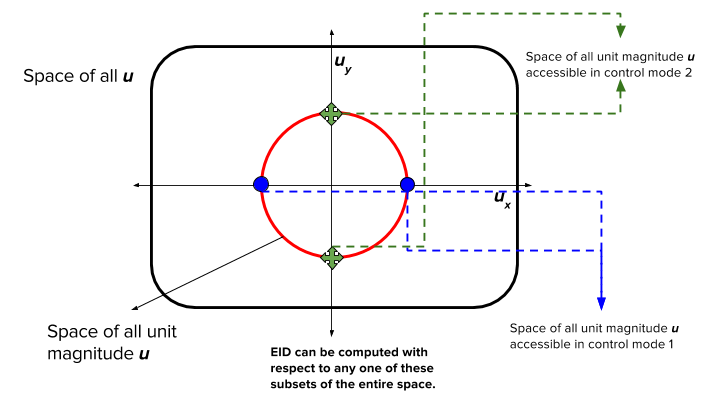
\includegraphics[width = 0.7\hsize, height = 0.26\vsize]{./figures/UH_SPACE.png}
	\vspace{-0.4cm}
	\caption{Illustration of subspaces of control command space.}
	\label{DM_FIG}
\end{figure}

Imagine that the virtual sensor that measures the ``entropy of confidence distributions'' is moving in the space of $\boldsymbol{u_h}$. 
In some parts of the space, the sensor readings will peak and in others they will not. This is akin to the electric field sensor getting close to the true spatial location of the goal in Miller et al. 

\subsubsection*{Math Formalism}

The entropy of the confidence distribution is the measurement model and can be written as, 

\begin{equation*}
e = \Upsilon(\boldsymbol{u_h}; \boldsymbol{x_r}, \boldsymbol{x_{g_1}},\dots,\boldsymbol{x_{g_n}}) + \delta, ~~~ \delta \sim \mathcal{N}(0, \sigma^2)
\end{equation*}

Let $\boldsymbol{x_r}, \boldsymbol{x_{g_1}},\dots,\boldsymbol{x_{g_n}}$ be denoted by $\boldsymbol{\Theta}$. The above equation then simplifies to 

\begin{equation*}
e = \Upsilon(\boldsymbol{u_h}; \boldsymbol{\Theta}) + \delta, ~~~ \delta \sim \mathcal{N}(0, \sigma^2)
\end{equation*}


where $\Upsilon$ is the entropy (negative of) of the confidence distribution and is a function of robot position and user control command. The robot and goal positions are treated as fixed parameters. 
Individual confidences are given as 
\begin{equation*}
c_{g^i} = \frac{1 + cos(\theta)}{2}
\end{equation*}
where 
\begin{equation*}
cos(\theta) = \frac{\boldsymbol{u_h}\cdot(\boldsymbol{x_{g^i}} - \boldsymbol{x_r})}{\norm{\boldsymbol{u_h}}\cdot\norm{\boldsymbol{x_{g^i}} - \boldsymbol{x_r}}}
\end{equation*}
Normalizing the confidences across the goals will result in a ``proxy'' probability distributions over goal confidences. 
\begin{equation*}
p(g^i) = \eta c_{g^i} ~~~,  \eta = \Sigma_{i = 1}^{n_g} c_{g^i}
\end{equation*}
$\eta$ is the normalization constant. 

Entropy of this distribution over goals is defined as 

\begin{equation*}
H(g) = -\Sigma_{i = 1}^{n_g}~p(g^i)~log[p(g^i)]
\end{equation*}
and
\begin{equation*}
\Upsilon(\boldsymbol{u_h}; \boldsymbol{\Theta}) = -H(g) = -(-\Sigma_{i = 1}^{n_g}~p(g^i)~log[p(g^i)])
\end{equation*}

It can be seen that $H(g)$ is a function of $\boldsymbol{u_h}$, given the robot position and goal positions (treated as fixed parameters). Given a set of goals and the form of the confidence function, entropy is a scalar defined for each robot position and user control command. 

\subsubsection*{Fisher Information Metric}
\begin{equation*}
\mathcal{I}_{i,j}(\boldsymbol{u_h}; \boldsymbol{\Theta}) = \frac{1}{\sigma^2}\frac{\partial^2\Upsilon(\boldsymbol{u_h};\boldsymbol{\Theta})}{\partial u_h^iu_h^j}
\end{equation*}

In order to compute the expected Fisher information density over different subspaces of the control command space we can compute the expectation of the above quantity over any subspace of interest $\mathcal{U}$. Each subspace (set of points) can correspond to a control mode. In the 2D case, with 1D control modes each mode contains two points; one corresponding to positive and negative unit magnitude control commands along the dimension of interest. 

\begin{equation*}
\Phi^{\mathcal{U}}_{i,j}(\boldsymbol{\Theta}) = \frac{1}{\sigma^2}\int_{u_{h} \in \mathcal{U}}\frac{\partial^2\Upsilon(\boldsymbol{u_h}; \boldsymbol{\Theta})}{\partial u_h^iu_h^j}p(\boldsymbol{u_h})d\boldsymbol{u_h}
\end{equation*}

Note that the above integral is a multidimensional integral, but has been written using a ``vector'' notation for convenience sake. 

\subsubsection*{Illustration of computation with 1D interface}

We will assume that only unit magnitude control commands are possible with the interface.

\noindent Control mode 1 ($\mathcal{U}_1$) corresponds to the set $[\{1,0\}, \{-1,0\}]$ and control mode 2 ($\mathcal{U}_2$) corresponds to the set $[\{0,1\}, \{0,-1\}]$. 

\noindent Let $p(\{0,1\}) = p(\{0,-1\}) = p(\{1,0\}) = p(\{-1,0\}) = 0.5$. 

%phi for U1 and phi for U2. EID for each. 
\noindent Computation of $\Phi^{\mathcal{U}_1}_{i,j}$:
\begin{equation*}
\Phi^{\mathcal{U}_1}_{i,j}(\boldsymbol{\Theta}) = \frac{1}{\sigma^2}\Big[^{}\left.\frac{\partial^2\Upsilon(\boldsymbol{u_h}; \boldsymbol{\Theta})}{\partial u_h^iu_h^j}\right\vert_{\boldsymbol{u_h} = \{1,0\}}p(\{1,0\}) + \left.\frac{\partial^2\Upsilon(\boldsymbol{u_h}; \boldsymbol{\Theta})}{\partial u_h^iu_h^j}\right\vert_{\boldsymbol{u_h} = \{-1,0\}}p(\{-1,0\})\Big]
\end{equation*}

\noindent Computation of $\Phi^{\mathcal{U}_2}_{i,j}$:

\begin{equation*}
\Phi^{\mathcal{U}_2}_{i,j}(\boldsymbol{\Theta}) = \frac{1}{\sigma^2}\Big[^{}\left.\frac{\partial^2\Upsilon(\boldsymbol{u_h}; \boldsymbol{\Theta})}{\partial u_h^iu_h^j}\right\vert_{\boldsymbol{u_h} = \{0,1\}}p(\{0,1\}) + \left.\frac{\partial^2\Upsilon(\boldsymbol{u_h}; \boldsymbol{\Theta})}{\partial u_h^iu_h^j}\right\vert_{\boldsymbol{u_h} = \{0,-1\}}p(\{0,-1\})\Big]
\end{equation*}

EID of $\mathcal{U}_1$ can be computed as $\text{det}(\bar{\Phi}^{\mathcal{U}_1}(\boldsymbol{\Theta}))$ and EID of $\mathcal{U}_2$ as $\text{det}(\bar{\Phi}^{\mathcal{U}_2}(\boldsymbol{\Theta}))$ with $\boldsymbol{\Theta}$ to be the current robot position and the goal positions. 	

If EID of $\mathcal{U}_1$ is greater than EID of $\mathcal{U}_2$ it implies that control mode 1 has greater disambiguation capability. 

\subsubsection*{Preliminary insights and issues}

This formulation seems to work the best compared to all others. There are certain numerical issues (divide by zero et cetera) that are problematic and are dealt with by making approximations to the control commands. The approximations do have an impact on the results, but they are minor I believe.  

Following are some of the ``point cloud'' plots which depicts the best control mode for different points in the workspace. Control mode 1 (red) controls the X axis, and mode 2 (blue) controls the Y Axis. 

\begin{figure}[h]
	\centering
	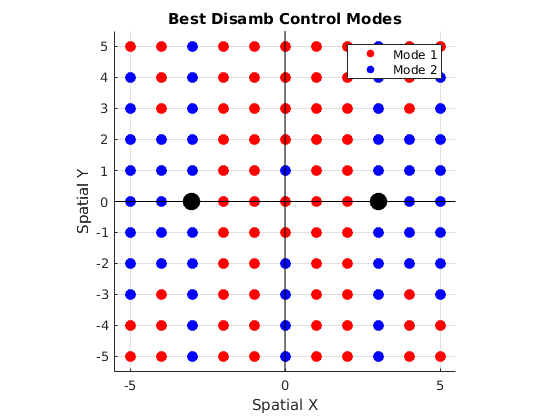
\includegraphics[width = 0.6\hsize, height = 0.25\vsize]{./figures/X_Config.png}
	\vspace{-0.4cm}
	\caption{Disambiguating control modes.}
%	\label{DM_FIG}
\end{figure}
\begin{figure}[h!]
	\centering
	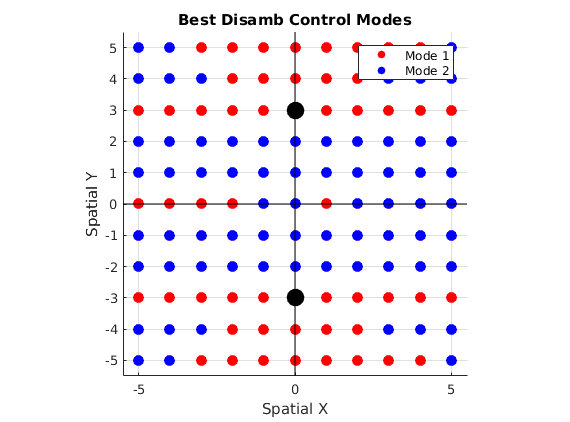
\includegraphics[width = 0.6\hsize, height = 0.3\vsize]{./figures/Y_Config.png}
	\vspace{-0.4cm}
	\caption{Disambiguating control modes.}
	%	\label{DM_FIG}
\end{figure}
\begin{figure}[h!]
	\centering
	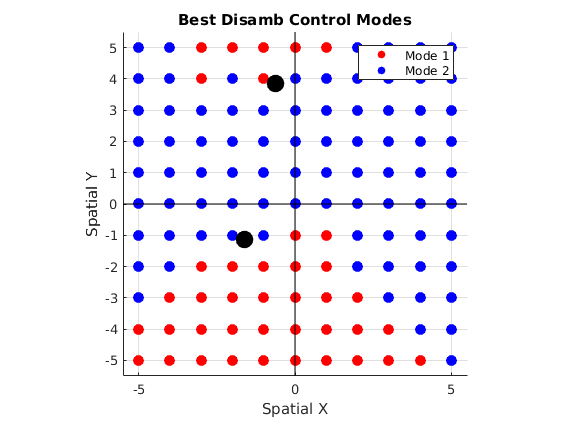
\includegraphics[width = 0.6\hsize, height = 0.27\vsize]{./figures/Config1.png}
	\vspace{-0.4cm}
	\caption{Disambiguating control modes.}
	%	\label{DM_FIG}
\end{figure}
\begin{figure}[h!]
	\centering
	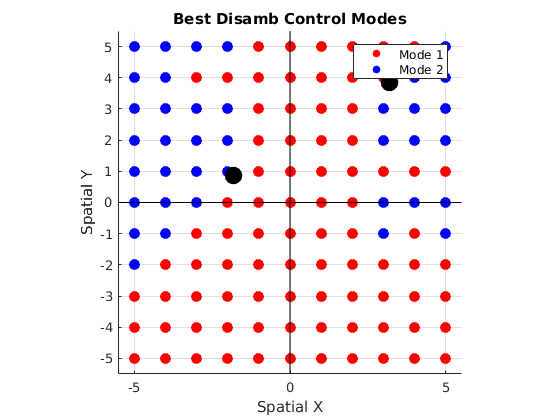
\includegraphics[width = 0.6\hsize, height = 0.27\vsize]{./figures/Config2.png}
	\vspace{-0.4cm}
	\caption{Disambiguating control modes.}
	%	\label{DM_FIG}
\end{figure}

\begin{figure}[h]
	\centering
	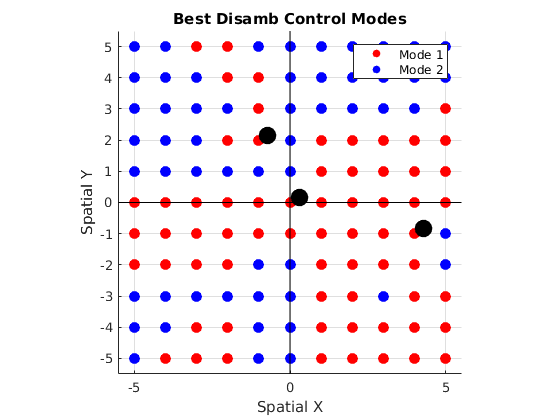
\includegraphics[width = 0.6\hsize, height = 0.27\vsize]{./figures/Config3.png}
	\vspace{-0.4cm}
	\caption{Disambiguating control modes.}
	%	\label{DM_FIG}
\end{figure}
\begin{figure}[h!]
	\centering
	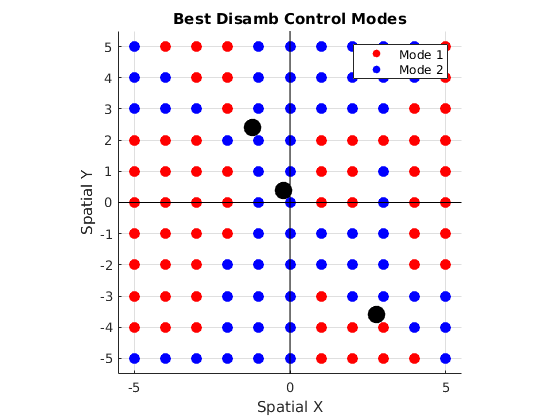
\includegraphics[width = 0.6\hsize, height = 0.25\vsize]{./figures/Config4.png}
	\vspace{-0.4cm}
	\caption{Disambiguating control modes.}
	%	\label{DM_FIG}
\end{figure}

\begin{figure}[h!]
	\centering
	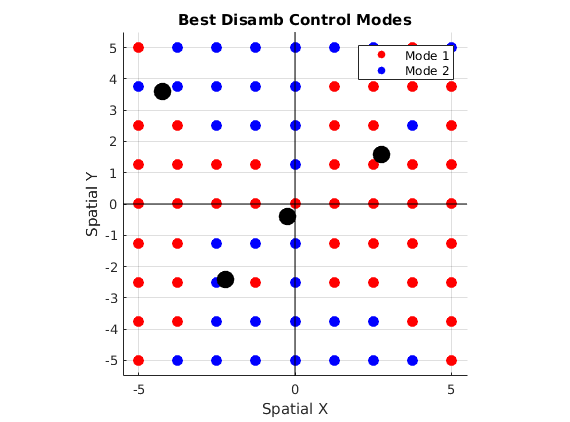
\includegraphics[width = 0.6\hsize, height = 0.3\vsize]{./figures/Config5.png}
	\vspace{-0.4cm}
	\caption{Disambiguating control modes.}
	%	\label{DM_FIG}
\end{figure}
\begin{figure}[h!]
	\centering
	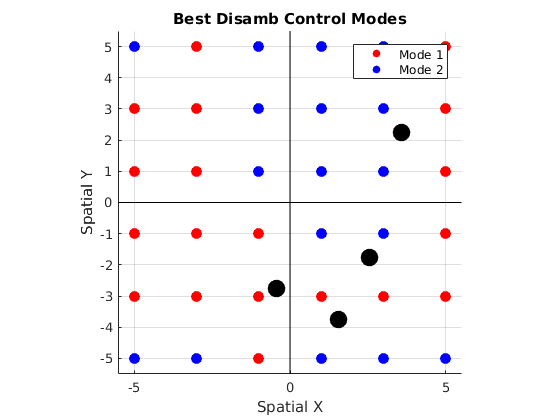
\includegraphics[width = 0.6\hsize, height = 0.3\vsize]{./figures/Config6.png}
	\vspace{-0.4cm}
	\caption{Disambiguating control modes.}
	%	\label{DM_FIG}
\end{figure}
\begin{figure}[h!]
	\centering
	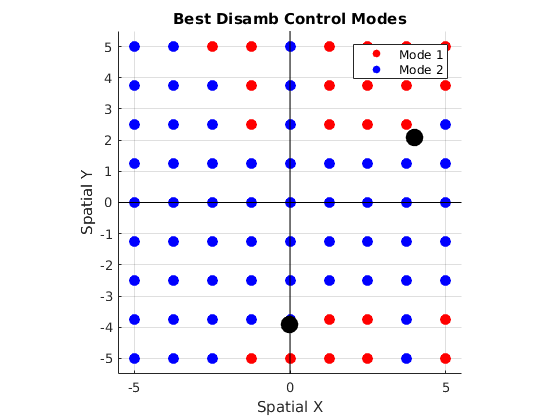
\includegraphics[width = 0.6\hsize, height = 0.3\vsize]{./figures/Config7.png}
	\vspace{-0.4cm}
	\caption{Disambiguating control modes.}
	%	\label{DM_FIG}
\end{figure}

\subsubsection*{Reflections}
\textit{``...The Fisher Information $\mathcal{I}(\theta, x)$ can be thought of as the amount of information a measurement provides at location $x$ for a given estimate of $\theta$...''}

\noindent\textit{``...Fisher information quantifies the ability of a random variable, in our case a measurement, to estimate an unknown parameter... }

In the light of the above statements from Todd's papers, how justifiable is our approach! 
\subsubsection*{References}
1. Silverman, Y., L. M. Miller, M. A. MacIver, and T. D. Murphey, "Optimal Planning for Information Acquisition", IROS 2013, 2013. 

\noindent 2. Miller, L. M., and T. D. Murphey, "Optimal Planning for Target Localization and Coverage Using Range Sensing", IEEE Int. Conf. on Automation Science and Engineering (CASE): 2015, pp. 501-508, 2015.  

\end{document}
